\chapter{Einleitung}
Die graphische Darstellung von Daten, das Diagramm, ist von grosser Bedeutung für die Gesellschaft. Man findet Diagramme überall: In etlichen Wissenschaften, wo sie nicht wegzudenken sind, in jeglichen Industrien, in Zeitungen, in Werbungen.

Das Ziel eines Diagramms ist die Vermittlung von Zusammenhängen und Informationen des dargestellten Datensatzes. Der Leser sollte sich mit den Daten auseinandersetzen können, ohne die Rohdaten (die gesammelten Daten, die in dem Diagramm dargestellt werden) betrachten zu müssen. Je nachdem wie das Diagramm graphisch umgesetzt wird, können verschiedene Zusammenhänge und Informationen des Datensatzes hervorgehoben oder in den Hintergrund gestellt werden, was einen Einfluss auf die Vermittlung einen Einfluss hat.

Im Informationszeitalter sind Daten von immer grösserer Bedeutung, der Datenfluss vergrössert sich ständig. Um Daten darstellen zu können, müssen sie zuerst gesammelt, sortiert und formatiert werden, bevor man mit der Auswertung beginnen kann. Das Sammeln von Daten stellt oftmals keine besondere Schwierigkeit dar, das Auswerten, Darstellen und Interpretieren ist eine Herausforderung.

Konventionell werden Diagramme in Zeitungen, Artikeln abgedruckt. Der Autor trifft Entscheidungen, wie die Daten in graphischer Form dargestellt werden und erstellt auf Basis dieser ein Diagramm. Nach dem Druck kann es vom Leser betrachtet werden, jedoch kann dieser die Darstellung nicht mehr verändern, das Diagramm ist statisch. Er hat darum keinen Einfluss, wie die Daten in diesem \textbf{statischen Diagramm} dargestellt und an ihn vermittelt werden.

Durch das Aufkommen von modernen Computern, Smartphones haben sich die Möglichkeiten zur Darstellung erweitert: Dem Nutzer ist es möglich, mit dem Diagramm zu interagieren. Unter anderem findet man in Online-Zeitschriften solche \textbf{dynamischen Diagramme}, welche Daten darstellen, die mit dem Artikel zu tun haben und interaktiv vom Nutzer bedient werden können. <beschreiben von den figures nytimes taxes und nytimes realestate>

\begin{figure}[htbp]
	\centering
	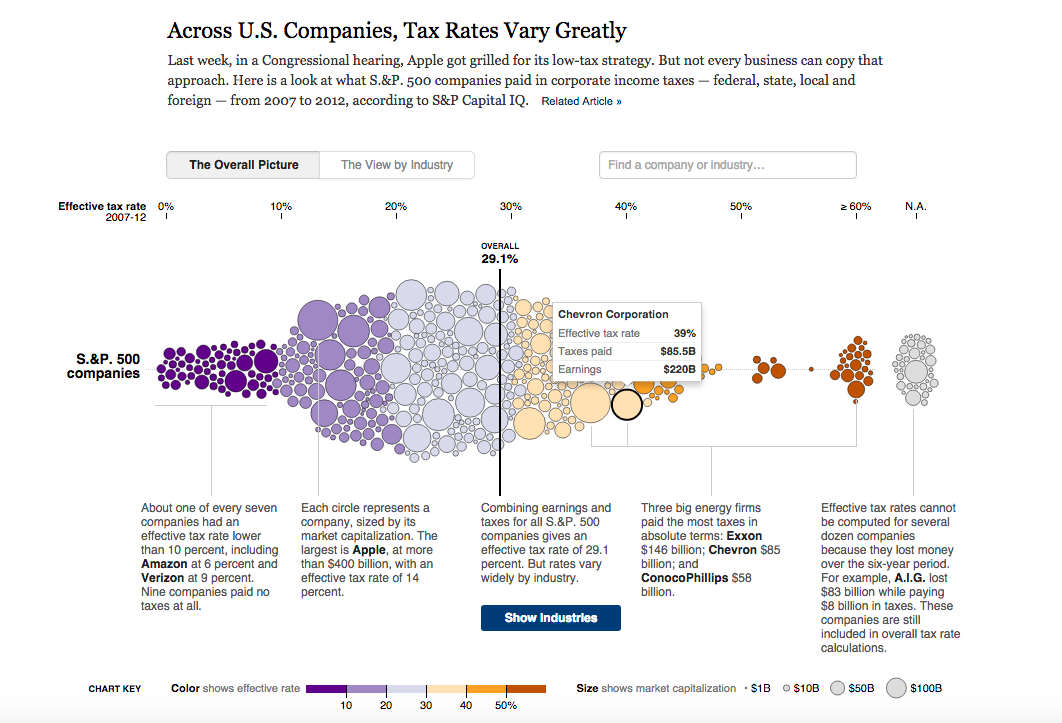
\includegraphics[width=1\linewidth]{images/nytimes-taxes}
	\caption[Bubble-Diagramm in der New York Times]{Eine Bubble-Diagramm, das die Höhe der Steuern darstellt, die verschiedene Firmen in den USA zahlen. \cite{nytimes-taxes}}
	\label{fig:nytimes-taxes}
\end{figure}

\begin{figure}[htbp]
	\centering
	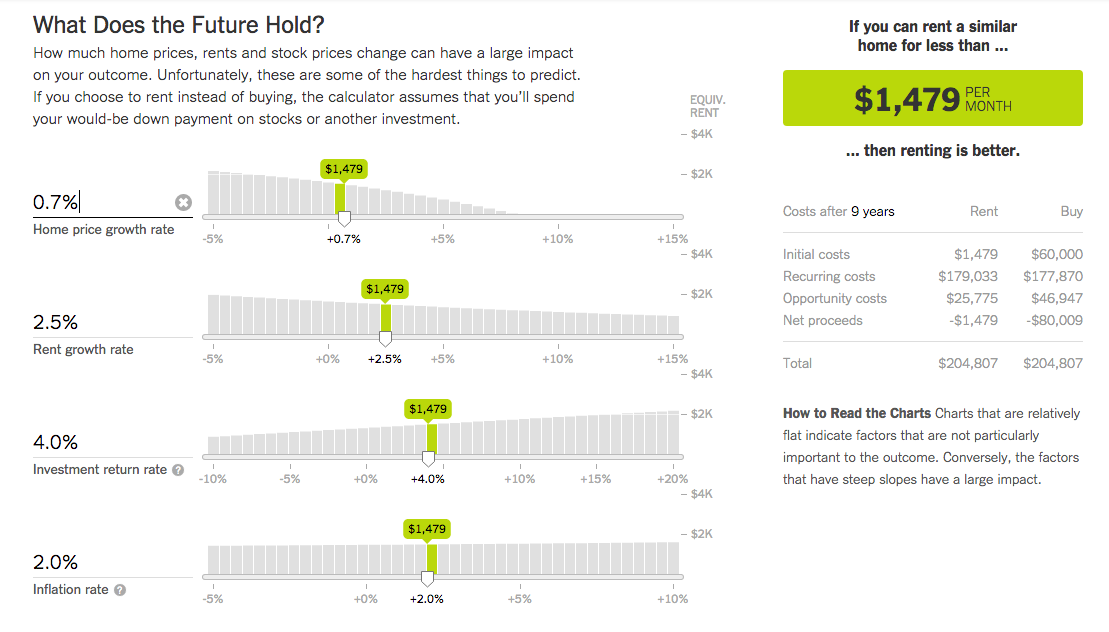
\includegraphics[width=1\linewidth]{images/nytimes-realestate}
	\caption[Interaktives Diagramm in der New York Times]{Interaktives Diagramm, das anzeigt, ob es bei bestimmten Konditionen der Kauf oder die Miete eines Hauses profitabler ist. \cite{nytimes-realestate}}
	\label{fig:nytimes-realestate}
\end{figure}

Diese Maturaarbeit wurde inspiriert von dem Artikel \textit{The Eyes Have It: A Task by Data Type for Information Visualizations} von B. Shneidermann \cite{shneiderman}. Der Artikel untersucht, wie ein Benutzer eine Programmoberfläche wahrnimmt und auf welche Weise er mit ihr interagiert. Auch beschreibt der Artikel, wie die Oberfläche aufgebaut sein sollte, damit der Benutzer sich im Programm orientieren kann, es versteht und ohne grossen Aufwand es bedienen kann. 

Die von Shneidermann beschriebenen Prinzipien für das Design von Benutzeroberflächen werden in dieser Arbeit berücksichtigt. Es werden interaktive, dynamische Diagramme entwickelt, die den Informationsertrag des Nutzers verbessern sollten. Er sollte sich mit den Daten effizienter auseinandersetzen können, besser verstehen und Spass an der Erkundung des Datensatzes haben \cite{shneiderman}.

\section{Wahl des Diagrammtyps}

Es gibt sehr viele Arten von Diagrammen, welche sich unterschiedlich für verschiedene Datentypen eignen. Diese Arbeit beschränkt sich auf einen Diagrammtyp, das Streudiagramm. Das Streudiagramm wird in der Wissenschaft als auch in anderen Medien oft verwendet. Es stellt beobachtete Wertepaare zweier Merkmale dar. Diese zwei Werte werden als Punkte in ein kartesisches Koordinatensystem eingetragen, welches zwei- oder mehrdimensional sein kann. Dadurch entsteht eine Menge vom Punkten. In der Praxis, falls ein Verlauf von Werten, zum Beispiel über eine Zeit, dargestellt werden will, werden die Punkte oft nicht gezeichnet und durch eine Linie verbunden.

Die Beschränkung der Arbeit auf ein einzigen Diagrammtyp ermöglicht, dass man auf sehr spezifische Aspekte des Arbeitsproduktes eingehen kann und nicht die Untersuchung generell formulieren muss.

\section{Technologie}

Die interaktiven Diagramme werden in der Praxis fast ausschliesslich für den Web-Browser entwickelt, Technologien wie HTML (für den Inhalt), CSS (für das Aussehen), SVG (für Vektorgrafiken), JavaScript (für die Berechnung) werden verwendet, diese ermöglichen die dynamische Manipulation durch den Nutzer. Der Prozess der Entwicklung in diesen Technologien wird grösstenteils im Kapitel \ref{chapter:praktischer_teil} dokumentiert.
